\chapter{Analyse des besoins et conception g\'en\'erale}
\label{chap:requirements}

\section*{Introduction}
Avant d'entamer l'impl\'ementation technique, il est primordial de d\'elimiter pr\'ecis\'ement le p\'erim\`etre fonctionnel et technique de la plateforme. Ce deuxi\`eme chapitre a pour vocation de sp\'ecifier les exigences fonctionnelles et non fonctionnelles, d'identifier les acteurs du syst\`eme, et de formaliser le backlog produit selon le cadre m\'ethodologique Agile Scrum. Nous pr\'esentons ensuite la conception g\'en\'erale \`a travers le diagramme de cas d'utilisation global et le mod\`ele conceptuel des donn\'ees m\'etier.

\section{Identification des acteurs}
Un acteur repr\'esente toute entit\'e humaine ou logicielle qui interagit directement avec le syst\`eme. L'architecture de notre plateforme de supervision t\'el\'ecom repose sur deux r\^oles utilisateurs humains ainsi que deux acteurs externes d\'etaill\'es dans le tableau~\ref{tab:acteurs}.

\begin{table}[H]
\centering
\begin{tabular}{|p{4.2cm}|p{9.8cm}|}
\hline
\textbf{Acteur} & \textbf{R\^ole et responsabilit\'es} \\
\hline
\textbf{Administrateur} & Supervise l'ensemble de la plateforme \`a l'\'echelle nationale. Il assure la gouvernance globale, g\`ere les comptes des Responsables de Zone, configure le d\'ecoupage spatial (polygones g\'eographiques), audite les logs d'activit\'e et acc\`ede \`a tous les indicateurs KPI strat\'egiques. \\
\hline
\textbf{Responsable de Zone} & Pilote les op\'erations au sein de son p\'erim\`etre territorial assign\'e (\textit{Zone-Scoped}). Il supervise la cartographie interactive (NRO, FDT, Contrats), re\c{c}oit les flux d'alertes en temps r\'eel, traite les r\'eclamations des abonn\'es enrichies par l'IA et analyse la saturation des \'equipements. \\
\hline
\textbf{Sondes R\'eseau (Syst\`eme Externe)} & Capteurs t\'el\'ecom et sondes optiques transmettant de mani\`ere continue les \'ev\'enements terrain (mesures de puissance, coupures de c\^ables, pannes d'\'equipements). \\
\hline
\textbf{Groq LPU Cloud (Service Externe)} & Service d'inf\'erence d'Intelligence Artificielle fournissant les capacit\'es LLM (Llama 3) \`a ultra-haute vitesse pour la classification, la priorisation et la recommandation d'actions sur les r\'eclamations. \\
\hline
\end{tabular}
\caption{Description d\'etaill\'ee des acteurs du syst\`eme}
\label{tab:acteurs}
\end{table}

\section{Sp\'ecification des exigences}

\subsection{Exigences fonctionnelles}
Le syst\`eme r\'epond \`a six grands ensembles d'exigences fonctionnelles :

\begin{enumerate}
    \item \textbf{Module Authentification \& Contr\^ole d'acc\`es (RBAC) :}
    \begin{itemize}
        \item Authentification s\'ecuris\'ee par identifiant/mot de passe avec g\'en\'eration de tokens JWT sign\'es.
        \item Contr\^ole d'acc\`es bas\'e sur les r\^oles (\texttt{AppRole.ADMIN} et \texttt{AppRole.RESPONSABLE\_ZONE}) et filtrage contextuel des donn\'ees selon la zone affect\'ee (\textit{Zone-Scoped Access Control}).
        \item Administration compl\`ete des utilisateurs (cr\'eation, modification, affectation de zone, activation/d\'esactivation, audit).
    \end{itemize}

    \item \textbf{Module R\'eseau \& Topologie Optique :}
    \begin{itemize}
        \item Gestion hi\'erarchique des entit\'es : Zones g\'eographiques, NRO, FDT, Contrats clients et C\^ables optiques.
        \item D\'etection et mise \`a jour dynamique des liaisons et de la topologie suite aux \'ev\'enements r\'eseau.
    \end{itemize}

    \item \textbf{Module Cartographie Interactive (SIG) :}
    \begin{itemize}
        \item Visualisation g\'eolocalis\'ee multi-couches avec tuiles cartographiques interactives.
        \item Filtrage dynamique par zone, type d'\'equipement, \'etat de fonctionnement et niveau de s\'ev\'erit\'e.
        \item Fiches d\'etaill\'ees en popups interactifs avec acc\`es direct aux m\'etriques op\'erationnelles.
    \end{itemize}

    \item \textbf{Module Temps R\'eel \& Notifications :}
    \begin{itemize}
        \item Ingestion continue des \'ev\'enements r\'eseau et d\'ecouplage asynchrone via BullMQ/Redis.
        \item Diffusion instantan\'ee des alertes et synchronisation automatique des interfaces clientes via WebSockets (Socket.IO).
        \item Centre de notifications avec historique, filtrage et accus\'es de lecture.
    \end{itemize}

    \item \textbf{Module Intelligence Artificielle \& Aide \`a la d\'ecision :}
    \begin{itemize}
        \item \textbf{IA R\'eclamations :} Analyse s\'emantique automatique du contenu textuel des r\'eclamations pour inf\'erer la cat\'egorie, la priorit\'e et une recommandation d'intervention.
        \item \textbf{IA Saturation NRO :} Analyse de la capacit\'e et du taux d'occupation des ports pour anticiper les risques de saturation.
    \end{itemize}

    \item \textbf{Module Tableaux de bord \& KPI :}
    \begin{itemize}
        \item Visualisation synth\'etique des indicateurs de performance (taux de disponibilit\'e, temps moyen de r\'esolution MTTR, r\'epartition des pannes par zone).
    \end{itemize}
\end{enumerate}

\subsection{Exigences non fonctionnelles}
Les exigences non fonctionnelles garantissent la robustesse et la p\'erennit\'e du syst\`eme en conditions r\'eelles de production :

\begin{table}[H]
\centering
\begin{tabular}{|p{3.5cm}|p{10.5cm}|}
\hline
\textbf{Cat\'egorie} & \textbf{Sp\'ecification technique} \\
\hline
\textbf{S\'ecurit\'e} & Chiffrement des mots de passe avec \textit{bcrypt}, transmission chiffr\'ee HTTPS/WSS, validation stricte des DTOs (\textit{class-validator} en mode whitelist), et stockage s\'ecuris\'e des jetons sur mobile via \textit{flutter\_secure\_storage}. \\
\hline
\textbf{Performance} & Temps de r\'eponse de l'API REST $< 200$\,ms sur les requ\^etes standards ; latence de diffusion WebSocket $< 100$\,ms ; indexation g\'eospatiale optimis\'ee \textit{2dsphere} sous MongoDB. \\
\hline
\textbf{Disponibilit\'e \& R\'esilience} & Traitement asynchrone des \'ev\'enements via Redis pour absorber les pics de charge ; int\'egration d'un \textit{Circuit Breaker} sur les appels d'inf\'erence LLM avec repli d\'eterministe (\textit{fallback}). \\
\hline
\textbf{Ergonomie} & Respect des principes \textit{Material Design 3}, affichage r\'eactif fluide ($60$\,FPS sur Flutter), et adaptation ergonomique aux contraintes d'utilisation sur le terrain. \\
\hline
\end{tabular}
\caption{Sp\'ecification des exigences non fonctionnelles}
\label{tab:non-fonct}
\end{table}

\section{Planification du projet : Product Backlog}
Conform\'ement \`a la m\'ethodologie Scrum, le backlog produit a \'et\'e structur\'e en User Stories r\'eparties sur 3 releases et 12 sprints (Tableau~\ref{tab:product-backlog}).

\begin{table}[H]
\centering
\small
\begin{tabular}{|c|c|p{3cm}|p{6.8cm}|c|}
\hline
\textbf{ID} & \textbf{Sprint} & \textbf{Fonctionnalit\'e} & \textbf{User Story} & \textbf{Priorit\'e} \\
\hline
\rowcolor{gray!15}
\multicolumn{5}{|c|}{\textbf{Release 1 : Socle technique, Authentification \& Gestion des Utilisateurs}} \\
\hline
1 & S0 & Cadrage \& Socle & En tant qu'\'equipe, initialiser les d\'ep\^ots, environnements et conventions & Haute \\
\hline
2 & S1 & Analyse des besoins & En tant qu'analyste, formaliser les exigences et les acteurs & Haute \\
\hline
3 & S2 & Conception technique & En tant qu'architecte, mod\'eliser le domaine et l'architecture & Haute \\
\hline
4 & S3 & Auth \& Users & En tant qu'utilisateur, m'authentifier et g\'erer les comptes selon les r\^oles & Haute \\
\hline
\rowcolor{gray!15}
\multicolumn{5}{|c|}{\textbf{Release 2 : Supervision r\'eseau, Cartographie interactive \& Temps r\'eel}} \\
\hline
5 & S4 & Mod\`ele Topologie & En tant que superviseur, g\'erer les zones, NRO, FDT et contrats & Haute \\
\hline
6 & S5 & Ingestion \& Temps r\'eel & En tant que syst\`eme, ing\'erer et diffuser les \'ev\'enements en temps r\'eel & Haute \\
\hline
7 & S6 & Cartographie Flutter & En tant que technicien, visualiser le r\'eseau sur carte interactive & Haute \\
\hline
8 & S7 & Dashboard \& Alertes & En tant qu'admin, analyser les KPI et g\'erer les notifications & Moyenne \\
\hline
\rowcolor{gray!15}
\multicolumn{5}{|c|}{\textbf{Release 3 : IA m\'etier, Tests, D\'eploiement \& Industrialisation}} \\
\hline
9 & S8 & IA R\'eclamations & En tant que superviseur, enrichir automatiquement les r\'eclamations & Moyenne \\
\hline
10 & S9 & IA Saturation NRO & En tant que d\'ecideur, anticiper la saturation des NRO & Moyenne \\
\hline
11 & S10 & Int\'egration \& Tests & En tant qu'\'equipe, valider l'int\'egration bout-en-bout et les tests & Haute \\
\hline
12 & S11 & D\'eploiement \& CI/CD & En tant qu'\'equipe, d\'eployer et documenter la version finale & Haute \\
\hline
\end{tabular}
\caption{Product Backlog global d\'etaill\'e par it\'erations Scrum}
\label{tab:product-backlog}
\end{table}

\section{Conception g\'en\'erale du syst\`eme}

\subsection{Diagramme de cas d'utilisation global}
La figure~\ref{fig:usecase-global} synth\'etise les interactions globales entre les acteurs et les principaux modules fonctionnels de la plateforme.

\begin{figure}[H]
 \centering
 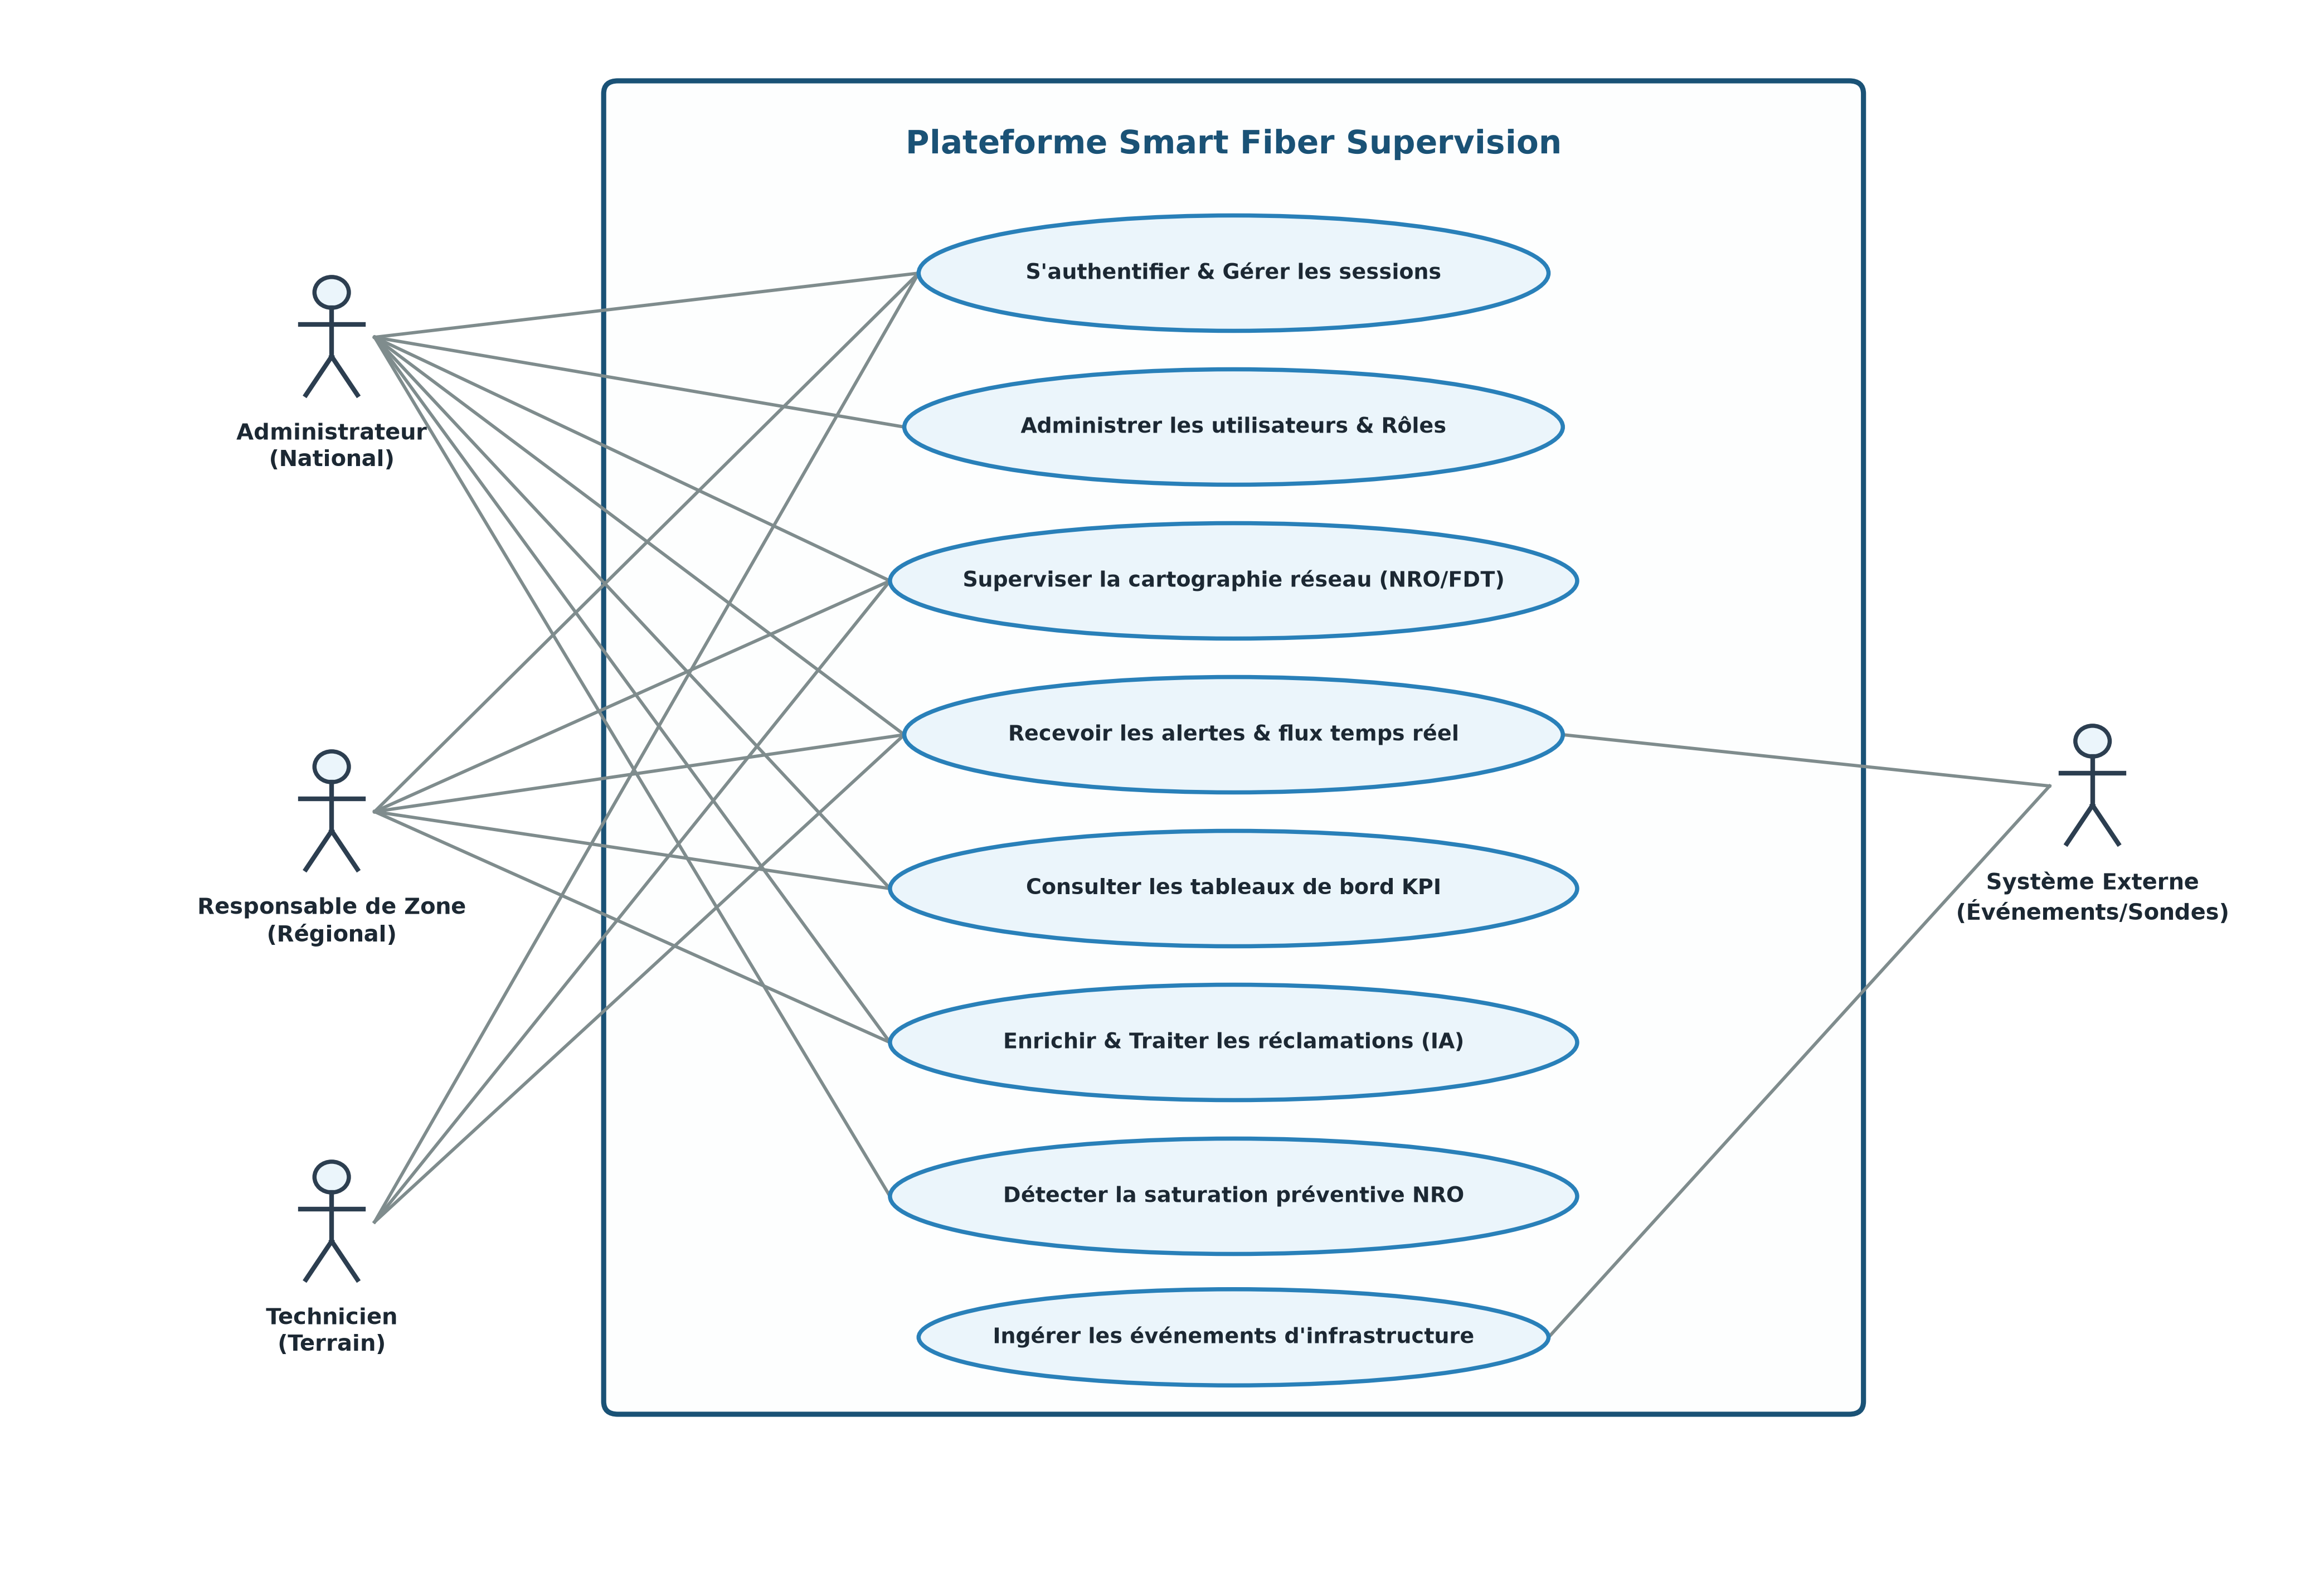
\includegraphics[width=15cm]{Images/usecase_global.png}
 \caption{Diagramme de cas d'utilisation global du syst\`eme}
 \label{fig:usecase-global}
\end{figure}

\subsection{Mod\`ele conceptuel de donn\'ees (Diagramme de classes global)}
La mod\'elisation conceptuelle du domaine t\'el\'ecom est illustr\'ee par la figure~\ref{fig:class-global}. Elle structure les relations entre les utilisateurs, les p\'erim\`etres g\'eographiques (\textit{Zone}), les \'equipements physiques optiques (\textit{NRO}, \textit{FDT}), les contrats abonn\'es et les r\'eclamations.

\begin{figure}[H]
 \centering
 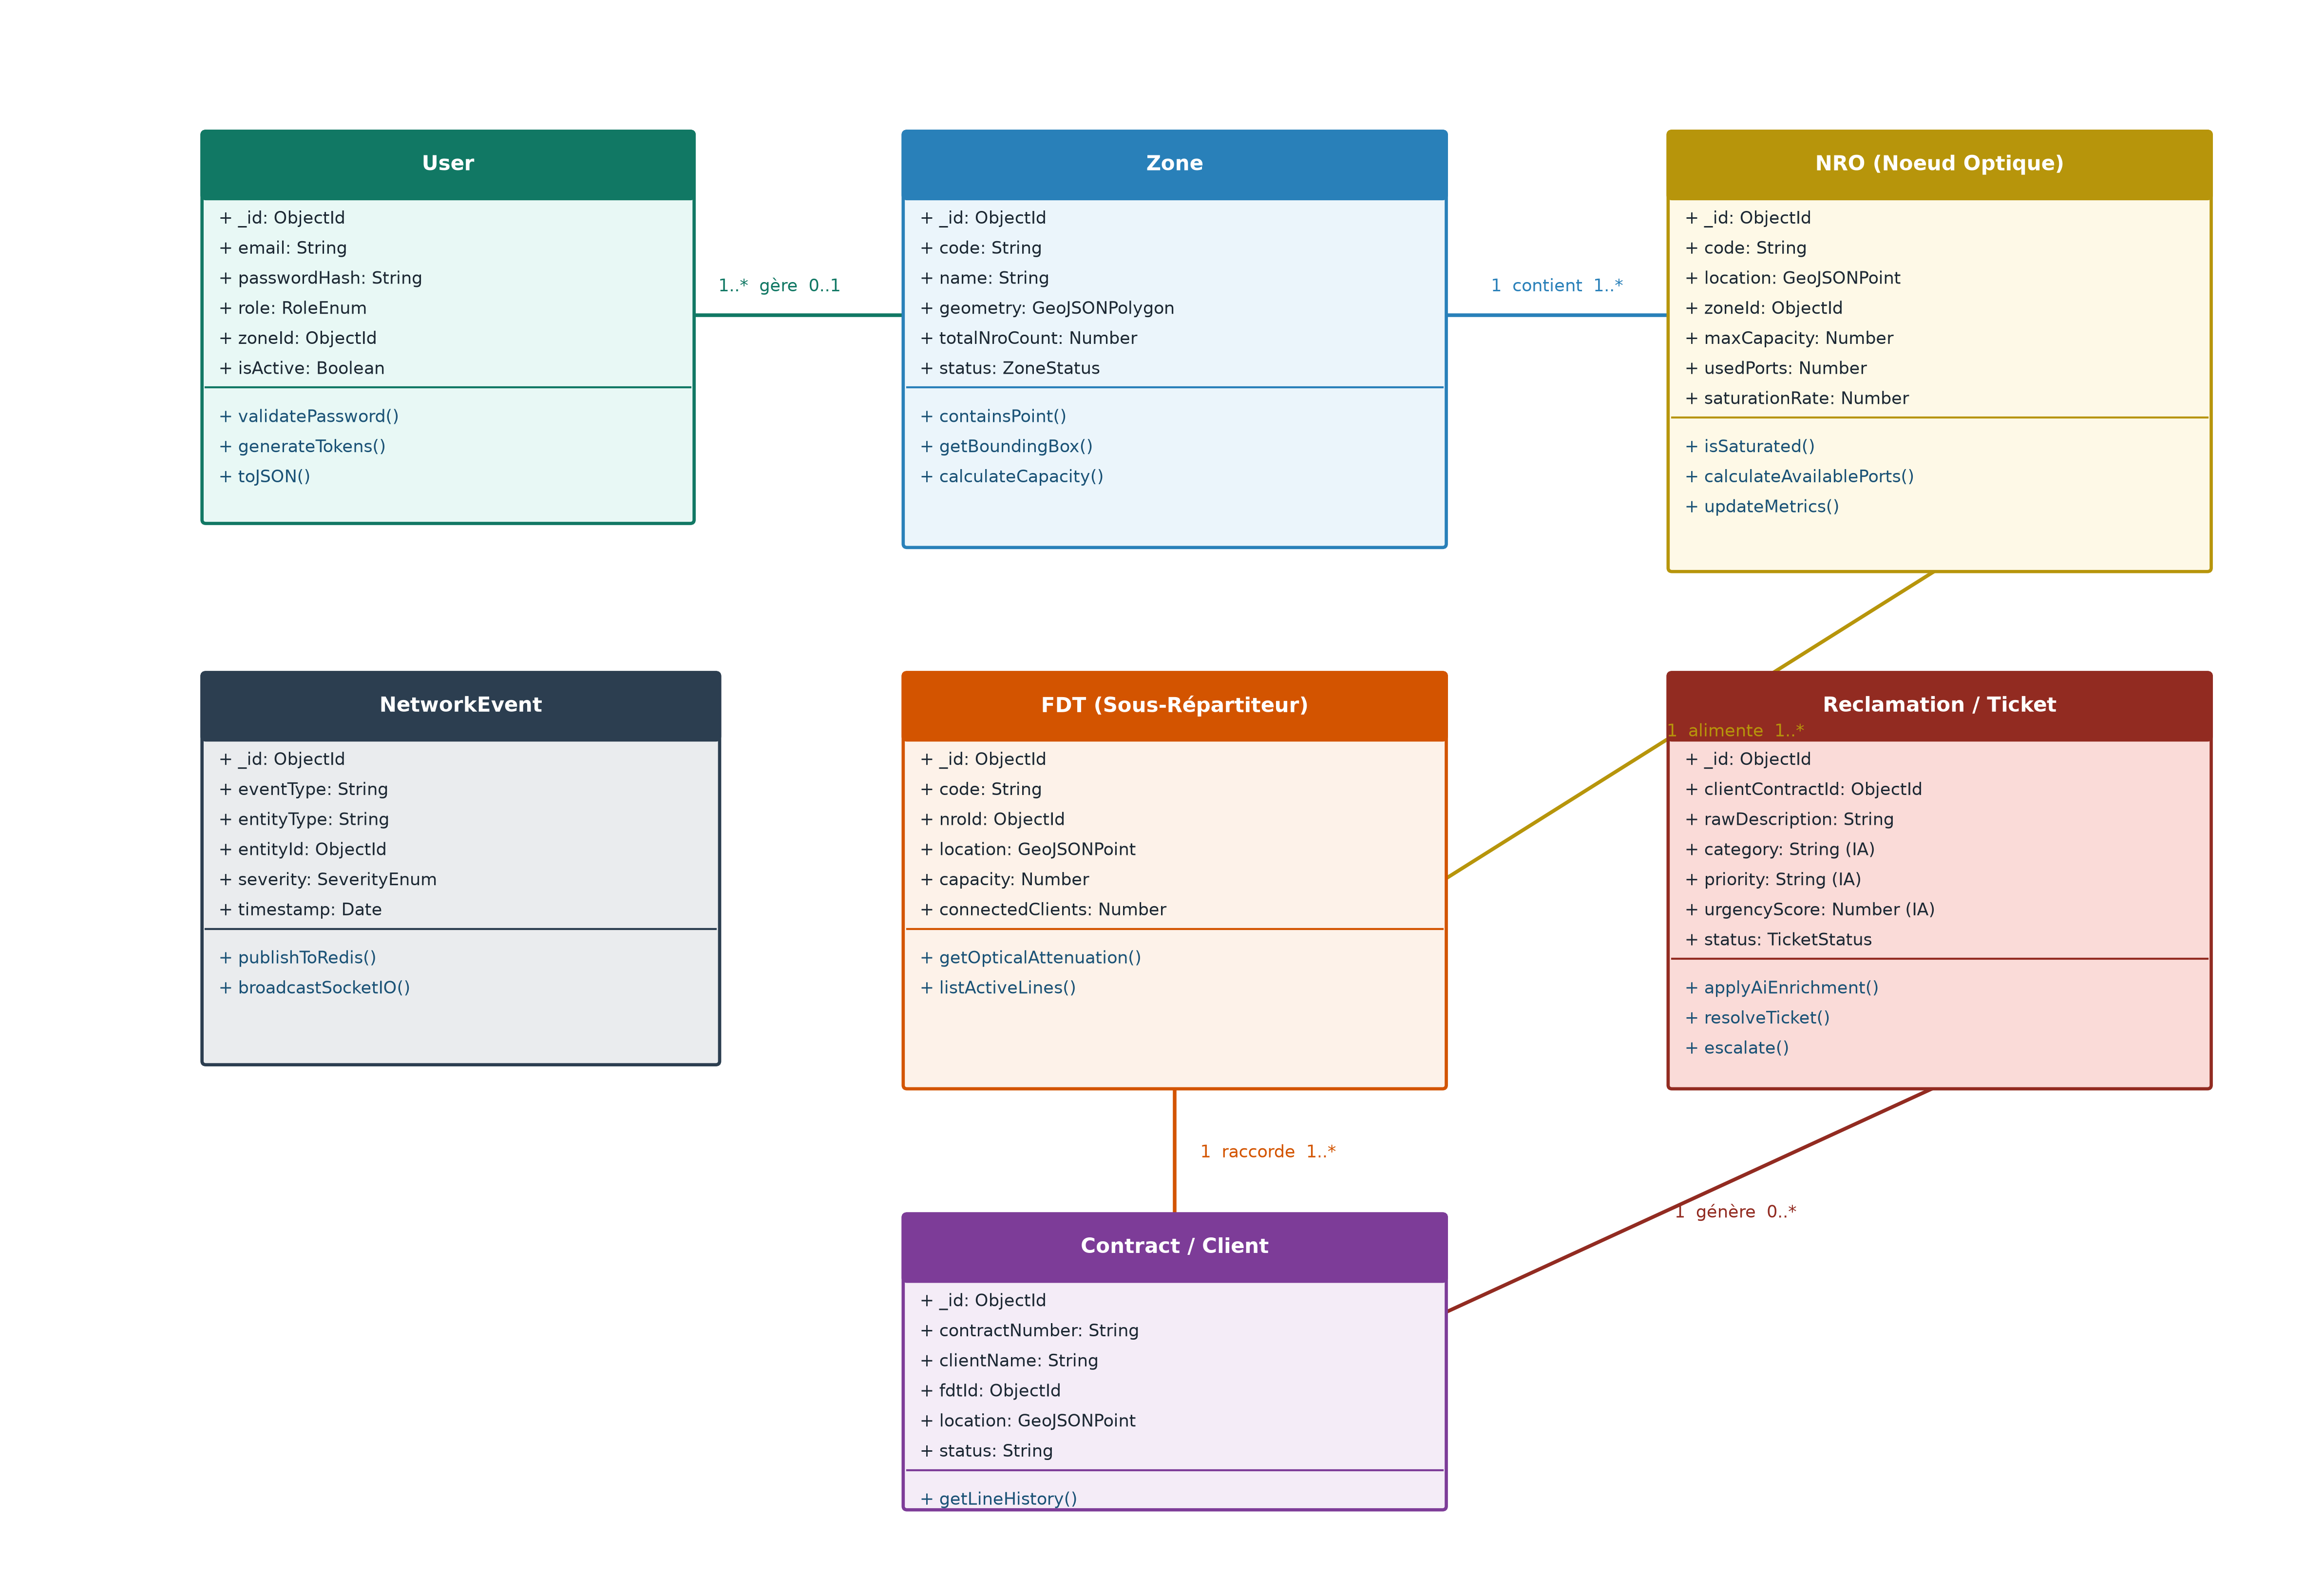
\includegraphics[width=15cm]{Images/class_global.png}
 \caption{Diagramme de classes conceptuel global du domaine m\'etier}
 \label{fig:class-global}
\end{figure}

\subsection{Vue d'ensemble de l'architecture fonctionnelle}
L'\'ecosyst\`eme logiciel s'articule autour de trois flux directeurs :
\begin{itemize}
    \item \textbf{Flux Administratif et Consultation (REST / HTTPS) :} Les requ\^etes de gestion CRUD et de chargement initial des couches cartographiques s'ex\'ecutent via l'API REST s\'ecuris\'ee par JWT.
    \item \textbf{Flux \'Ev\'enementiel et Alertes (WebSockets / WSS) :} Les changements d'\'etats r\'eseau et nouvelles r\'eclamations sont pouss\'es instantan\'ement vers l'application mobile.
    \item \textbf{Flux Asynchrone \& IA :} Les traitements lourds (analyse s\'emantique LLM, \'evaluation de la capacit\'e des NRO) sont d\'ecoupl\'es via les files BullMQ afin de garantir une disponibilit\'e maximale.
\end{itemize}

\section*{Conclusion}
Ce chapitre a permis de d\'efinir rigoureusement les besoins fonctionnels et non fonctionnels, d'identifier les r\^oles des acteurs et de structurer le backlog Scrum du projet. La conception globale a \'etabli les mod\`eles conceptuels de r\'ef\'erence. Les trois chapitres suivants pr\'esentent en d\'etail la r\'ealisation technique des trois releases du projet.